\input{/Users/daniel/github/config/preamble.sty}
\input{/Users/daniel/github/config/thms-eng.sty}
\bibliographystyle{alpha}

\begin{document}

\begin{minipage}{\textwidth}
	\begin{minipage}{1\textwidth}
		\hfill Daniel González Casanova Azuela
		
		{\small Prof. Sergey Galkin\hfill\href{https://github.com/danimalabares/ms}{github.com/danimalabares/ms}}
	\end{minipage}
\end{minipage}\vspace{.2cm}\hrule
\vspace{1em}
{\Huge Minimal Surfaces}

\tableofcontents

\section{Class 1}

\subsection{Intro}

Minimal surfaces started with Lagrange, at 19 years old, more than 250 years old, when he communicated with Euler. Something is minimized. For Lagrange, this was the area functional with respect to euclidean metric \((dx)^2+(dy)^2+(dz)^2\). He was looking for surfaces that \textit{locally} minimize area. He wrote differential equations characterizing this property.

\subsection{Definition}

\[\begin{tikzcd}
&\mathbb{R}^3=\mathbb{R}^3_{x,y}\perp \mathbb{R}_z\\
\Sigma\arrow[rr,"\pi \circ j:=f_L"]\arrow[ur,"i"]&&\arrow[ul,"\mathbb{R}^2",swap]
\end{tikzcd}\]
The idea is that if \(L \in T_p \Sigma\), then \(f_L\) is locally a diffeorphism around \(p\). {\color{6}dani: So I think that decomposition of \(\mathbb{R}^3\) depends on \(L\).} By inverse function theorem, locally there exists a function \(\varphi(x,y)\) wuch that \(\Sigma=\Gamma_\varphi=\{(x,y,z): z=\varphi(x,y)\}\).

\begin{example}\leavevmode
A sphere is locally seen ass \(z=\sqrt{1-x^2-y^2} \).
\end{example}

\(\Omega \subset \mathbb{R}^2\) some region. Then consider a function that puts the boundary of the region in \(\mathbb{R}^3\) (it's the height function): \(\varphi: \overline{\Omega}\to \mathbb{R}\), \(\varphi|_{\partial\Omega}\). Then minimization of area becomes a PDE on \(\varphi\).

This PDE is historically the first Euler-Lagrange Equation (=equations of motion). Now there's a lot of generalizations of this in classical field theory also.hj n

\section{Class 2}

Lagrange's PDE - nonlinear PDE. From \cite{salsa}:
\[\operatorname{div}\left(\frac{\nabla u}{\sqrt{1+|\nabla u|^2} }\right) =0\]
Laplace equation 
\[\Delta x_i=0\]
and its nonhomogeneous version Poisson equation \[\Delta f=\rho \in \Omega^{2}(\Sigma)\]
\textbf{Rk.} you can think of laplacian on a surface as giving a 2-form by multipliyng by \(\operatorname{Vol}\), this will allow you to integrate. The point is that solution exists  \(\iff\) \([\rho] = 0 \in H^{2}(\Sigma,\mathbb{R})\). If \(\Sigma\) is not compact then there's always a solution. So  \(\Sigma\) compact \(\iff\) \(\int_\Sigma\rho=0\).

So when thinking of Riemann surfaces/complex analysis, if you have \(\Sigma_{(u,v)} \xrightarrow{\varphi}\mathbb{R}^n\) minimal, where \(x_i(u,v)\), then \(x_i\) is a harmonic function wr.t. \(\varphi^* g_{\mathbb{R}^n}\).

\begin{thing4}{Three ways to study minimal surfaces}\leavevmode
\begin{enumerate}
\item \(\sim\) PDE. Colding-Codazzi textbook.
\item Complex analysis/geometry/Riemannsurfaces/practice. Flourished in \(19^{\text{th} }\) century.
\item Geometric measure theory. Very popular these days. Back to Lebesgue (who invented Lebesgue integral when investigating minimal surfaces).
\end{enumerate}
\end{thing4}

Now we comment J. Simons who is the same from Chern-Simons and so many institutions and grants that go by the name Simons.


\begin{thing6}{Result}\leavevmode
In \(\mathbb{R}^3\) there are no closed (compact, without boundary) minimal surfaces.
\end{thing6}

So we look for things with boundary. So from the PDE point of view we look for some boundary condition. This is also called ``plateau problem", which was solved in the 1930's.

\begin{example}\leavevmode
Schwarz minimal surface:
\begin{figure}[H]
	\centering
	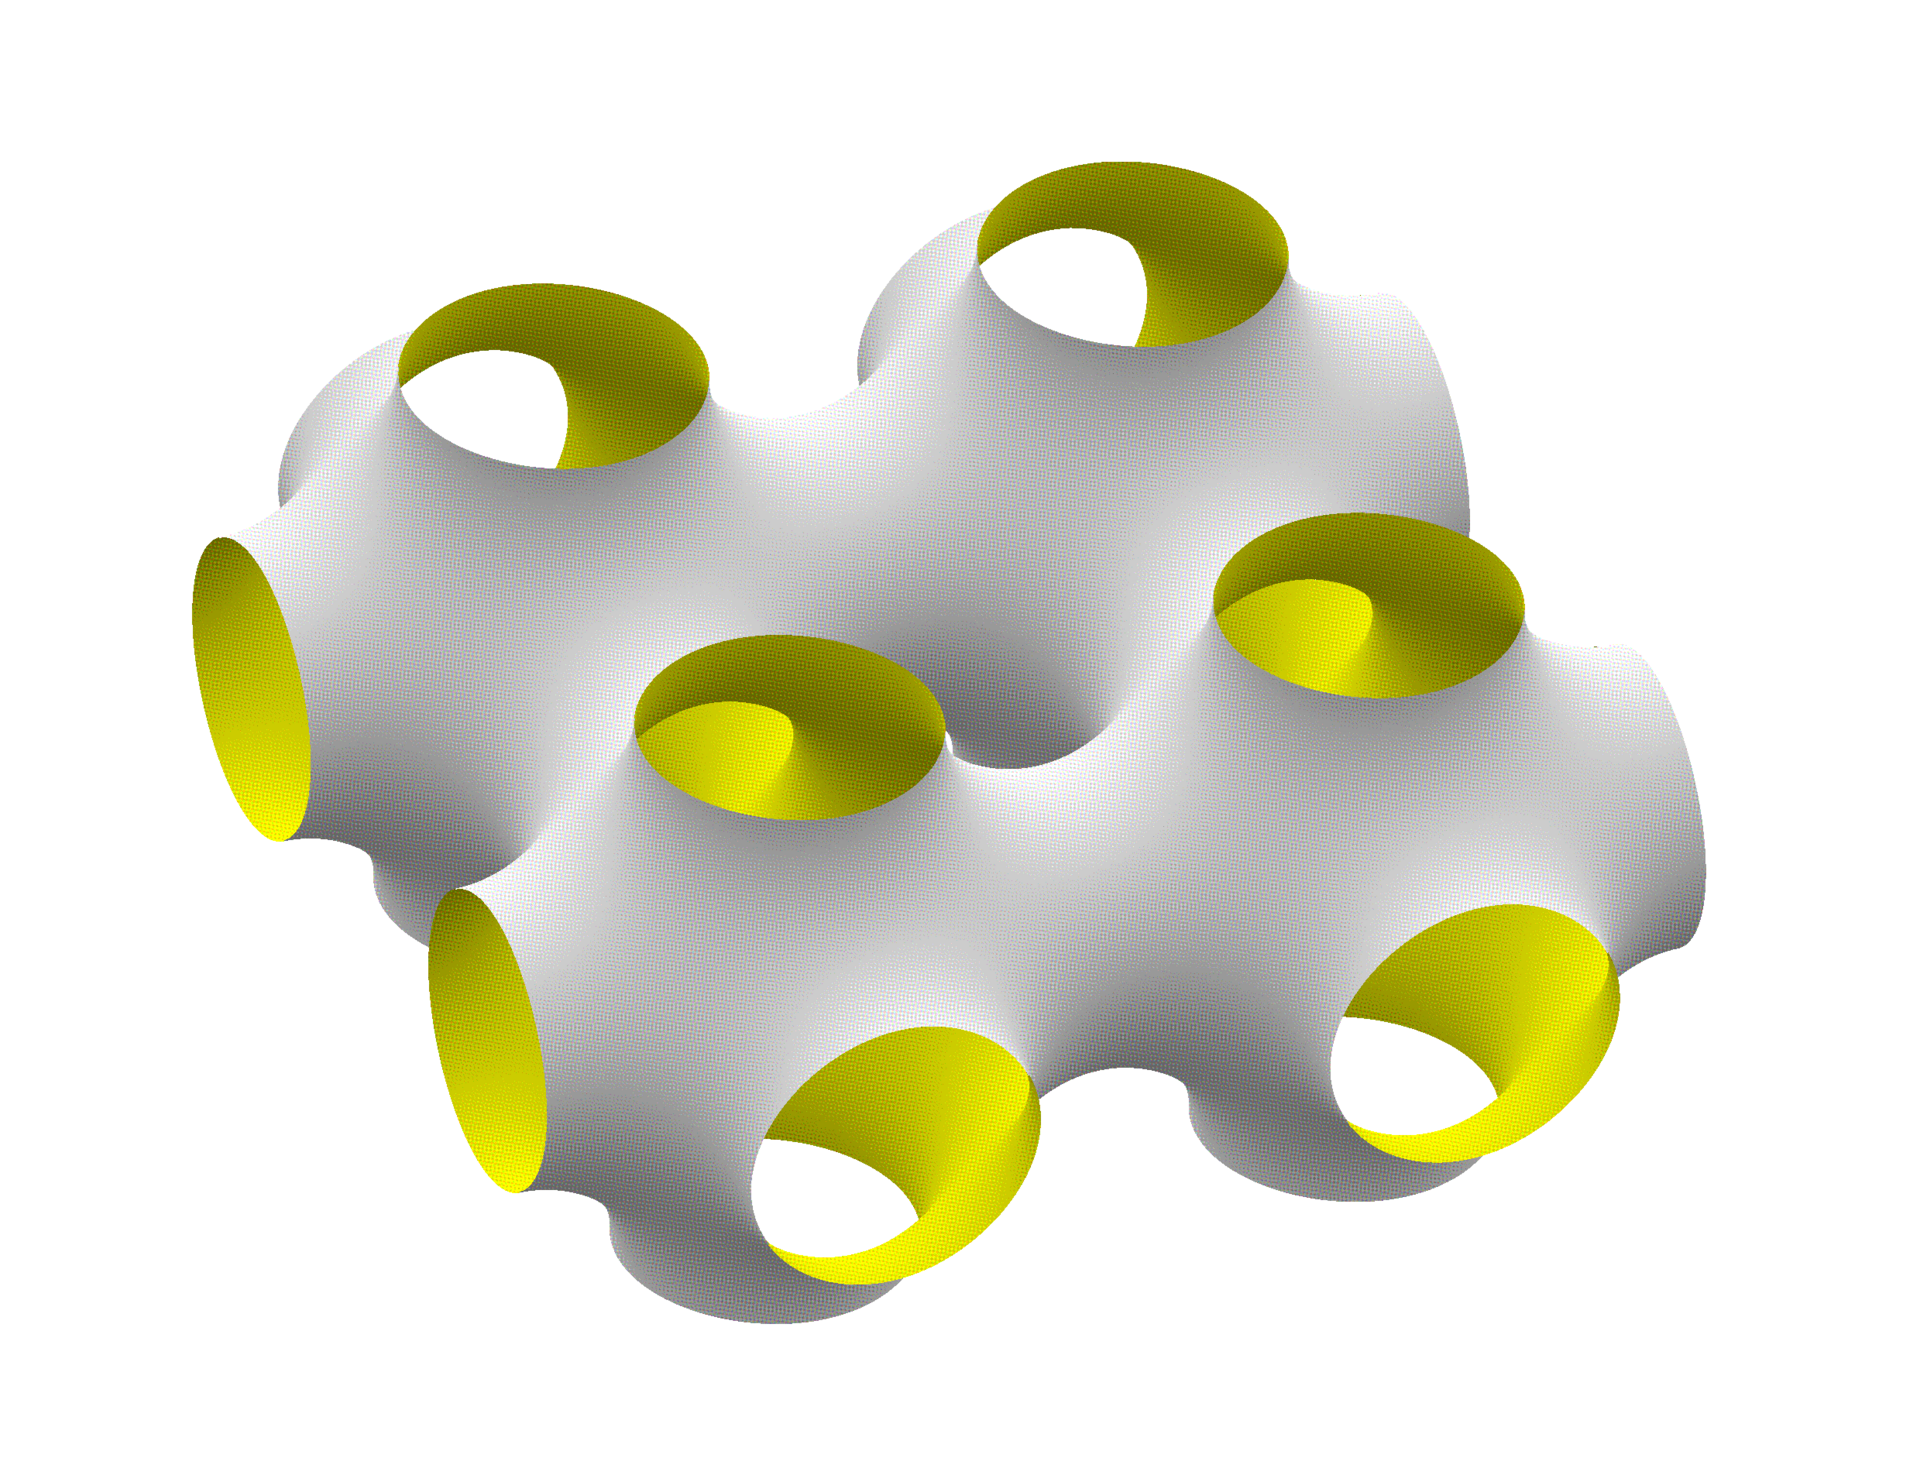
\includegraphics[width=0.5\textwidth]{fig1}
\end{figure}
You can think of this as put inside 3-torus \(\mathbb{T}^3\overset{\operatorname{def}}{=}\mathbb{R}^3/\mathbb{Z}^3\).
\end{example}

\begin{example}\leavevmode
Enneper surface.
\iffalse\begin{figure}[H]
	\centering
	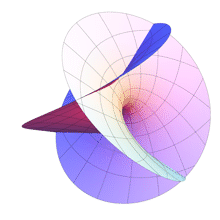
\includegraphics[width=.5\textwidth]{fig2.png}
\end{figure}\fi
\end{example}

*We saw several other examples* In conclusion, minimal surfaces exist and you can see some of them.

\subsection{Basic objects}

Consider
\[M^{(m)}\overset{f}{\hookrightarrow }N^{(n)}=\mathbb{R}^n,\qquad x_1,\ldots,x_n\]
It has a differential
\[T_pM \longrightarrow T_{f(p)}N=\mathbb{R}^n\]
which is a linear map. Now take local coordinates \(D \subset M\), \((u_1,\ldots,u_n)\). Then \(f \) is locally fiven by a functions of \(m\) variables
\begin{align*}
	x_1(u_1,\ldots,u_m)\\
	\vdots \\
	x_n(u_1,\ldots,u_m)
\end{align*}
while \(df_p\) is represented by a \(m\times n\) matrix
\[\left(\frac{\partial x_i}{\partial u_J}\right) ,\qquad  i=1,\ldots,n, j=1,\ldots,m\]
If \(N^{(n)}\cong M^{(m)}\times \mathbb{R}^{n-m}\) and \(f= \operatorname{id}_M \times \varphi\) (so \(M = \Gamma_\varphi\) a graph of \(\varphi\). Then we get a matrix
\[\begin{pmatrix} \operatorname{Id} & * \end{pmatrix} \]
Now look again at \(M \overset{f}{\hookrightarrow }N\). We can pull back the metric of \(N\), which is a symmetric tensor, getting a metric on \(M\). ({\color{6}dani: because \(f\) is immersion=differential is injective).}

So let's try to see how this metric looks like. The pullback metric should of course be something of the kind
\[\sum g_{j j'} du_j du_{j'}\]
now since \(g= \sum (dx_i)^2\) is euclidean metric we get
\[\sum \left(\sum \frac{\partial x^i}{\partial u_j}du_j\right)^2 \]
so that
\[g_{j_1j_2}= \sum \frac{\partial x^i}{\partial u_{j_1}}\frac{\partial x^i}{\partial u_{j_2}}\]
So if this matrix is \(G\) and \(J\) is the jacobian of \(f\) we just get
\[G=J^{\mathbf{T}}J\]

\begin{remark}\leavevmode
We could also just define a metric on \(M\) by putting those coefficient functions and create s symmetric 2-tensor.
\end{remark}
Now consider
\[\bar{g} :=\det(g_{ij})\]
if \(\bar{g}\neq 0 \) then matrix  \((g_{ij})\) is invertible, so it has inverse \((g^{ij})\).

\begin{thing8}{Definition/Proposition}\leavevmode
\(f\) is \textit{\textbf{regular}} in a point \(p\) if any of these equivalent conditions hold:
\begin{enumerate}
\item \(\bar{g}\neq 0\).
\item \(\bar{g}>0\).
\item Vectors \(\left(df_p\right) \left(\frac{\partial }{\partial u_i}\right) \) are linearly independent.
\end{enumerate}
\end{thing8}

\begin{proof}\leavevmode
\end{proof}

\begin{defn}[Cotangent and tangent space]\leavevmode
For a local system of coordinates we can define
\[\Omega_{\mathbb{R}^n}:=\left<dx^{(1)},\ldots,dx^{(n)}\right>\]
as the space generated by the differentials of the coordinate functions. Then we define
\[T_{\mathbb{R}^n}:=\left<\frac{\partial }{\partial x^{(1)}},\ldots,\frac{\partial }{\partial x^{(n)}}\right>\]
as generated by the dual basis of the cotangent basis.
\end{defn}

\subsection{Volume of a submanifold of \(\mathbb{R}^n\)}

Consider \(U,V\) vector spaces and
\[\begin{tikzcd}
	U \arrow[r,"T"]& U \arrow[ r,"\sharp_g"]\arrow[r,"\cong",swap]&  U^{\vee}\arrow[r,"T^*"]&  U^{\vee}
\end{tikzcd}\]
where \(g\) is a metric on \(V\). Then the composition of all this is just the same as the pullback metric on \(U\)! 
\[T^*  \circ \sharp_g \circ T=\sharp_{T^*g}:U \to U^{\vee}\]
Now apply \(\Lambda^{m}\) to get another commutative diagram
\[\begin{tikzcd}
	\Lambda^{m}U \arrow[ r,"\Lambda^{m}T"]\arrow[rrr,bend right,"\bar{g}"]\arrow[d,equals]&\Lambda^{m}V\arrow[r,"\Lambda^{m}\sharp g"]&\Lambda^{m}V^{\vee}\arrow[ r,"\Lambda^{m}T^{\vee}"]&  \Lambda^{m}U^{\vee}\arrow[d,equals]\\
	\mathbb{R}& & & \mathbb{R}
\end{tikzcd}\]
and then the composition here gives us
\[\bar{g}=\sum_{1\leq  j_1\leq \ldots \leq j_m \leq n}\left(\det\left(\frac{\partial x^{j_k}}{\partial u_i}\right) \right) ^2\]

Let \(v_1,\ldots,v_n\) be a basis of \(U\) and \(e_1,\ldots,e_n\) another basis. Let \(V\) be a matrix that takes one basis to another. Then
\[G=V^{\mathbf{T}}V\]
\[\implies \det G= \det(V)^2\implies \bar{g}(p)=\operatorname{Vol}_M\Big((df)_p\left(\frac{\partial }{\partial u_1}\right),\ldots,(df)_p\left(\frac{\partial }{\partial u_n}\right) \Big)^2 \]

\begin{defn}[Volume of \(M \overset{f}{\hookrightarrow }\mathbb{R}^n\)]\leavevmode
 \[\operatorname{Vol}M=\int_M\sqrt{\det g}du_1\ldots du_m \]
\end{defn}

Which takes us to the problem of volume minimzation.

Then followed some computation of the minors of
\[\begin{pmatrix} 1&0&z_x\\0&1&z_y \end{pmatrix}\ldots \]


\clearpage\bibliography{bib.bib}
\end{document}
